% !TEX root = ../../main.tex
\subsection{Applying Bayes' Theorem to Particle Decays and Branching Ratios}
\label{sec:analysis:bayes}
We examine a newly discovered particle which was found to be able to decay in two different ways. 
This means there are two different decay channels, α and β. 
The probability \( \falpha \) for decay α to happen is called the \quotedef{branching ratio}.

We can recognize that each decay is a Bernoulli trial, because of two reasons. 
First, there are exactly two outcomes: it can \emph{either} go to channel α \emph{or} to channel β. 
Second, the probabilities of a decay going to either channel are fixed.
Therefore, the probabilities for one decay are
\begin{subequations}
\begin{gather}
    P(\upalpha) = \falpha, \\
    P(\mathrm{β}) = 1 - \falpha.
\end{gather}
\end{subequations}

When the number of trials \( N \) is fixed, a series of \emph{statistically independent} Bernoulli trials is called a \define{Bernoulli process}.
A Bernoulli process is described by the binomial distribution,
\begin{equation}
    \label{eq:bayes:binomial_distribution}
    p(k \given N, \falpha) = \binom{N}{k} \, \falpha^k \, (1 - \falpha)^{N - k}.
\end{equation}
Here, \( N \) is the total number of decays, \( k \) is the number of \quotedef{successes}, i.e. the number of decays to channel α, and \( \falpha \) is the probability of a decay going to the α channel.
Therefore, with a fixed number \( N \) of observed decays, the number of decays to one of the channels (e.g. α) follows a binomial distribution.

\subsubsection{Bayes' Theorem}
\label{sec:analysis:bayes:bayes_theorem}
Bayes' Theorem tells us how to update our beliefs about a parameter of a distribution when we get new information from measurements.
In this case the model is a Bernoulli process, described by the binomial distribution in \autoref{eq:bayes:binomial_distribution}.
The binomial distribution is dependent on the probability \( \falpha \), which is our parameter.

We start with some notion of what this parameter might be.
This is codified in the prior probability distribution, \( \pi(\falpha) \).
In the Bayesian sense the function gives the level of confidence (probability) that a certain value for \( \falpha \) is correct.
If we make a set of \( \vec{N} \) observations of \( \vec{k} \) decays to α, we can calculate the likelihood \( L(\vec{k} | \vec{N}, \falpha) \) of these observations given our model,
\begin{equation}
    \label{eq:bayes_theorem:likelihood_definition}
    L(\vec{k} | \vec{N}, \falpha) = \prod_{i} p(k_i \given N_i, \falpha).
\end{equation}
Since our model is a Bernoulli process, we find that our likelihood will follow the proportionality
\begin{equation}
    \label{eq:bayes_theorem:likelihood_proportionality}
    L(\vec{k} | \vec{N}, \falpha) \propto \prod_{i = 1}^n \falpha^{k_i} (1 - \falpha)^{N_i - k_i} = \falpha^k (1 - \falpha)^{N - k},
\end{equation}
where we defined \( k = \sum_i k_i\) and \( N = \sum_i N_i \), respectively the total number of successes and trials.
Finally, we can calculate the probability of the parameter taking on a certain value given our observations,
\begin{equation}
    \label{eq:bayes_theorem:posterior}
    p(\falpha | \vec{k}, \vec{N}) = \frac{L(\vec{k} | \vec{N}, \falpha) \cdot π(\falpha)}{\int L(\vec{k} | \vec{N}, \falpha) \cdot π(\falpha) \difl{\falpha}}.
\end{equation}
This \emph{Posterior Probability Distribution} over the possible values of the parameter \( \falpha \) lets us estimate what the true value of the original system is.

\subsubsection{Calculating the Posterior Probability Distribution}
For small \( N \), we can explicitly calculate the posterior distribution of \( \falpha \).
If a single decay was measured going to α, the likelihood is simply \( L(\upalpha | \falpha) = \falpha \).%
\footnote{Technically, this represents an abuse of our notation as defined above.
Correct would be writing \( L(k = 1 | N = 1, \falpha) \), or even \( L(\vec{k} | \vec{N}, \falpha) \) where \( \vec{k} = (k_1) \), \( \vec{N} = (N_1) \), and \( N_1 = k_1 = 1 \).}
Because we have no reason to weight our distribution before the first piece of data, the prior distribution will be flat and limited to the interval \( [0, 1] \), because probabilities must be between \num{0} and \num{1}. 
Therefore, \( \forall \falpha \in [0, 1]\colon \pi(\falpha) = 1 \) and the posterior is
\begin{equation}
    p(\falpha | \upalpha) = \frac{\falpha \cdot 1}{\int_0^1 \falpha \cdot 1 \difl{\falpha}} = 2 \falpha.
    \label{eq:bayes_theorem:posterior_1_decay}
\end{equation}

If another measurement is made, we can use \autoref{eq:bayes_theorem:posterior_1_decay} as the new prior and calculate the likelihood using \autoref{eq:bayes_theorem:likelihood_definition}.
This approach of starting with a prior, making observations, then calculating the posterior to become the next prior is called \quotedef{updating beliefs}.
It is very logical and useful.

Often the necessary integrals are only numerically integrable, which means lots of time and computing power are needed to find the result.
Here the concept of a \quotedef{conjugate prior} comes in handy.
The general idea is to find a function specified by some set of \quotedef{hyperparameters} which serves as a prior.
These hyperparameters should be such that the calculated posterior will also be of the same form, just with different values for the hyperparameters.

For the Bernoulli process, which is described by a binomial distribution, this conjugate prior is called the beta distribution.
It has the form
\begin{equation}
    π(\falpha) = \frac{\falpha^{\alpha - 1} (1 - \falpha)^{\beta - 1}}{\Beta(\alpha, \beta)}, \quad \falpha \in [0,1]
\end{equation}
where \( \alpha \) and \( \beta \) are the hyperparameters and \( \Beta \) is the beta function. 
The beta function normalizes the beta distribution.
Using \autoref{eq:bayes_theorem:likelihood_proportionality}, we check the proportionality of \autoref{eq:bayes_theorem:posterior},
\begin{equation}
    p(\falpha | \vec{k}, \vec{N}) \propto \falpha^k (1 - \falpha)^{N - k} \falpha^{α - 1} (1 - \falpha)^{β - 1} = \falpha^{α + k - 1} (1 - \falpha)^{β + N - k - 1},
\end{equation}
and see that the posterior indeed becomes a beta distribution with parameters \( α' = α + k \) and \( β' = β + N - k \).

While the calculations of the posterior are analytically solvable for small \( N \), we implement the more robust method using conjugate priors. 
The beta distribution is implemented in the \verb|scipy.stats| package, which we will use in our implementation of the calculations.
Our choice of a uniform prior can be modelled with the hyperparameters \( α = β = 1 \).
For a single measurement, our calculation will show that this method is equivalent to the analytic function \( p(\falpha|\upalpha) = 2 \falpha \).
Using the conjugate prior method, we graph the prior and posterior probability distributions of \( \falpha \) in \autoref{fig:bayes_theorem:prior_posterior_one_alpha_decay}.
\begin{figure}
    \centering
    \begin{subfigure}{.4\textwidth}
        \centering
        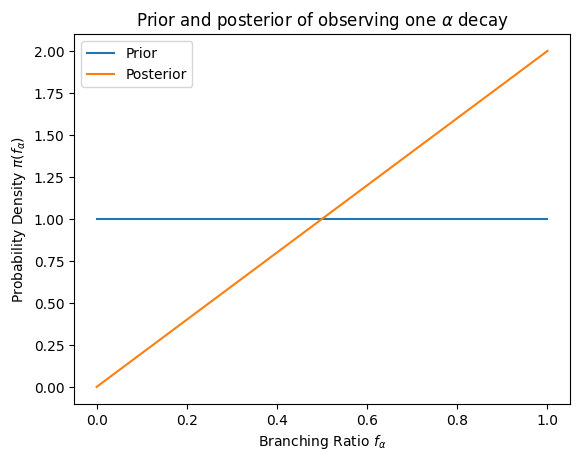
\includegraphics[width=.9\textwidth]{Graphs/Bayes/one_decay.png}
        \caption{Given One α Decay}
        \label{fig:bayes_theorem:prior_posterior_one_alpha_decay}
    \end{subfigure}
    \begin{subfigure}{.4\textwidth}
        \centering
        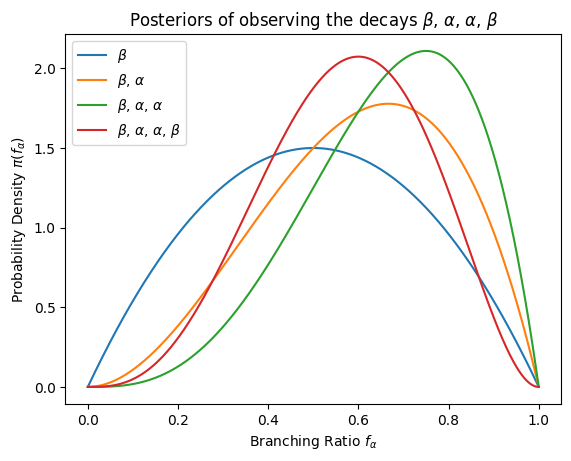
\includegraphics[width=.9\textwidth]{Graphs/Bayes/multiple_decays.png}
        \caption{Given Multiple Decays}
        \label{fig:bayes_theorem:posteriors_2_to_5}
    \end{subfigure}
    \begin{subfigure}{.4\textwidth}
        \centering
        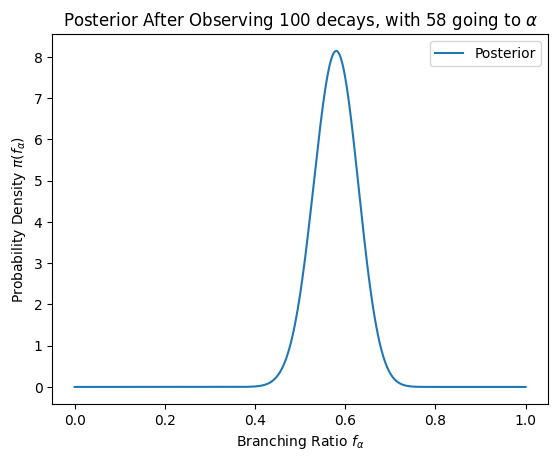
\includegraphics[width=.9\textwidth]{Graphs/Bayes/100_decays.png}
        \caption{Given \num{100} Data Points}
        \label{fig:bayes_theorem:posterior_100_decays}
    \end{subfigure}
    \caption{(Prior and) Posterior Probability Distribution of \( \falpha \).}
    \label{fig:bayes_theorem:posteriors}
\end{figure}

Now we are given four further measurements, \( \vec{k} = (\mathrm{β}, \upalpha, \upalpha, \mathrm{β}) \).
We set the previous result as the new prior and calculate the new posteriors after one more of these measurements, until we have used all measurements to inform the posterior.
To see the evolution of our knowledge about the parameter \( \falpha \), in \autoref{fig:bayes_theorem:posteriors_2_to_5} we graph the posteriors after each new data point is added.

Because of our robust implementation for calculating posteriors, we can now use the same code to calculate the posterior after a large number of decays.
In this case, we are given a total of \( n = \num{100} \) decays, with \num{58} going to α.
The posterior is given in \autoref{fig:bayes_theorem:posterior_100_decays}.